%%%%%%%%%%%%%%%%%%%%%%%%%%%%%%%%%%%%%%%%%%%%%%%%%%%%%%%%%%%%%%%%%%%%%%%%%%%%%%%%
% TUM-Vorlage: Präsentation
%%%%%%%%%%%%%%%%%%%%%%%%%%%%%%%%%%%%%%%%%%%%%%%%%%%%%%%%%%%%%%%%%%%%%%%%%%%%%%%%
%
% Rechteinhaber:
%     Technische Universität München
%     https://www.tum.de
% 
% Gestaltung:
%     ediundsepp Gestaltungsgesellschaft, München
%     http://www.ediundsepp.de
% 
% Technische Umsetzung:
%     eWorks GmbH, Frankfurt am Main
%     http://www.eworks.de
%
%%%%%%%%%%%%%%%%%%%%%%%%%%%%%%%%%%%%%%%%%%%%%%%%%%%%%%%%%%%%%%%%%%%%%%%%%%%%%%%%


%%%%%%%%%%%%%%%%%%%%%%%%%%%%%%%%%%%%%%%%%%%%%%%%%%%%%%%%%%%%%%%%%%%%%%%%%%%%%%%%
% Zur Wahl des Seitenverhältnisses bitte einen der beiden folgenden Befehle
% auskommentieren und den ausführen lassen:
\documentclass[t]{beamer}
\usepackage[
    orientation=landscape,
    size=custom,
    width=25.4,
    height=19.05,
    scale=0.63 % erzeugt 16pt Schriftgröße
]{beamerposter}

\newcommand{\PraesentationSchriftgroesseSehrGross}{\fontsize{30}{45}}
\newcommand{\PraesentationSchriftgroesseGross}{\fontsize{22}{33}}
\newcommand{\PraesentationSchriftgroesseNormal}{\fontsize{16}{29}}
\newcommand{\PraesentationSchriftgroesseKlein}{\fontsize{12}{18}}
\newcommand{\PraesentationSchriftgroesseDreizeiler}{\fontsize{7}{10}}
\newcommand{\PraesentationSchriftgroesseAufzaehlungszeichen}{\fontsize{10}{8}}

\newcommand{\PraesentationAbstandAbsatz}{22.1pt}
\newcommand{\PraesentationPositionKorrekturOben}{0cm}
\newcommand{\PraesentationBeispieleSchriftgroessen}{30 | 22 | 16 | 12}
\documentclass{scrlttr2} % Dokumentenklasse: KOMA-Skript Letter

% Anpassbare Kopf- und Fußzeilen für KOMA-Skript:
%\usepackage{scrlayer-scrpage}

\usepackage[utf8]{inputenc} % Textkodierung: UTF-8
\usepackage[T1]{fontenc} % Zeichensatzkodierung

\usepackage{calc} % Berechnungen

\usepackage[ngerman]{babel} % Deutsche Lokalisierung
\usepackage{graphicx} % Grafiken
\usepackage[absolute]{textpos} % Positionierung

% Silbentrennung:
\usepackage{hyphenat}
%\tolerance 2414
%\hbadness 2414
%\emergencystretch 1.5em
%\hfuzz 0.3pt
%\widowpenalty=10000     % Hurenkinder
%\clubpenalty=10000      % Schusterjungen
%\vfuzz \hfuzz

% Euro-Symbol:
\usepackage[gen]{eurosym}
\DeclareUnicodeCharacter{20AC}{\euro{}}

% Schriftart Helvetica:
\usepackage[scaled]{helvet}
\renewcommand{\familydefault}{\sfdefault}

\usepackage{mathptmx} % skalierbare Formelschriften
\usepackage{tabto} % Tabulatoren
\usepackage{lastpage} % Letzte Seitenzahl auslesen
\usepackage{xstring} % Textmanipulation
\usepackage{setspace} % anpassbare Zeilenabstände

\usepackage{bookmark} % Lesezeichen

% Unterdrückung layoutbedingter Warnungen
\usepackage[immediate]{silence}
\WarningFilter[layout]{latex}{Reference `LastPage'} % Gesamtseitenzahl
\WarningFilter[layout]{lastpage}{Rerun to get the references right} % Gesamtseitenzahl
\WarningFilter[layout]{latex}{Label(s) may have changed.} % Referenz auf letzte Seite
\WarningFilter[layout]{textpos}{environment textblock* not in vertical mode} % Positionierung Seitenzahl
\WarningFilter[layout]{latex}{There were undefined references}


% Debugging:
%\DeactivateWarningFilters[layout] % Unterdrückte Warnungen einschalten
%\usepackage{layout} % Layout-Informationen
%\usepackage{printlen} % Längenwerte ausgeben
 % Seitenverhältnis 4:3
% %\documentclass[aspectratio=169]{beamer}
\documentclass[t,aspectratio=169]{beamer}
\usepackage[
    orientation=landscape,
    size=custom,
    width=25.4,
    height=14.2875,
    scale=0.5
]{beamerposter}

\newcommand{\PraesentationSchriftgroesseSehrGross}{\fontsize{25}{38}}
\newcommand{\PraesentationSchriftgroesseGross}{\fontsize{18}{27}}
\newcommand{\PraesentationSchriftgroesseNormal}{\fontsize{14}{21}}
\newcommand{\PraesentationSchriftgroesseKlein}{\fontsize{11}{17}}
\newcommand{\PraesentationSchriftgroesseDreizeiler}{\fontsize{7}{10}}
\newcommand{\PraesentationSchriftgroesseAufzaehlungszeichen}{\fontsize{10}{8}}

\newcommand{\PraesentationAbstandAbsatz}{18pt}
\newcommand{\PraesentationPositionKorrekturOben}{-1cm}
\newcommand{\PraesentationBeispieleSchriftgroessen}{25 | 18 | 14 | 11}
\documentclass{scrlttr2} % Dokumentenklasse: KOMA-Skript Letter

% Anpassbare Kopf- und Fußzeilen für KOMA-Skript:
%\usepackage{scrlayer-scrpage}

\usepackage[utf8]{inputenc} % Textkodierung: UTF-8
\usepackage[T1]{fontenc} % Zeichensatzkodierung

\usepackage{calc} % Berechnungen

\usepackage[ngerman]{babel} % Deutsche Lokalisierung
\usepackage{graphicx} % Grafiken
\usepackage[absolute]{textpos} % Positionierung

% Silbentrennung:
\usepackage{hyphenat}
%\tolerance 2414
%\hbadness 2414
%\emergencystretch 1.5em
%\hfuzz 0.3pt
%\widowpenalty=10000     % Hurenkinder
%\clubpenalty=10000      % Schusterjungen
%\vfuzz \hfuzz

% Euro-Symbol:
\usepackage[gen]{eurosym}
\DeclareUnicodeCharacter{20AC}{\euro{}}

% Schriftart Helvetica:
\usepackage[scaled]{helvet}
\renewcommand{\familydefault}{\sfdefault}

\usepackage{mathptmx} % skalierbare Formelschriften
\usepackage{tabto} % Tabulatoren
\usepackage{lastpage} % Letzte Seitenzahl auslesen
\usepackage{xstring} % Textmanipulation
\usepackage{setspace} % anpassbare Zeilenabstände

\usepackage{bookmark} % Lesezeichen

% Unterdrückung layoutbedingter Warnungen
\usepackage[immediate]{silence}
\WarningFilter[layout]{latex}{Reference `LastPage'} % Gesamtseitenzahl
\WarningFilter[layout]{lastpage}{Rerun to get the references right} % Gesamtseitenzahl
\WarningFilter[layout]{latex}{Label(s) may have changed.} % Referenz auf letzte Seite
\WarningFilter[layout]{textpos}{environment textblock* not in vertical mode} % Positionierung Seitenzahl
\WarningFilter[layout]{latex}{There were undefined references}


% Debugging:
%\DeactivateWarningFilters[layout] % Unterdrückte Warnungen einschalten
%\usepackage{layout} % Layout-Informationen
%\usepackage{printlen} % Längenwerte ausgeben
 % Seitenverhältnis 16:9
%%%%%%%%%%%%%%%%%%%%%%%%%%%%%%%%%%%%%%%%%%%%%%%%%%%%%%%%%%%%%%%%%%%%%%%%%%%%%%%%


%%%%%%%%%%%%%%%%%%%%%%%%%%%%%%%%%%%%%%%%%%%%%%%%%%%%%%%%%%%%%%%%%%%%%%%%%%%%%%%%
%%%%%%%%%%%%%%%%%%%%%%%%%%%%%%%%%%%%%%%%%%%%%%%%%%%%%%%%%%%%%%%%%%%%%%%%%%%%%%%%
% TUM-Vorlage: Personenspezifische Informationen
%%%%%%%%%%%%%%%%%%%%%%%%%%%%%%%%%%%%%%%%%%%%%%%%%%%%%%%%%%%%%%%%%%%%%%%%%%%%%%%%
%
% Rechteinhaber:
%     Technische Universität München
%     https://www.tum.de
% 
% Gestaltung:
%     ediundsepp Gestaltungsgesellschaft, München
%     http://www.ediundsepp.de
% 
% Technische Umsetzung:
%     eWorks GmbH, Frankfurt am Main
%     http://www.eworks.de
%
%%%%%%%%%%%%%%%%%%%%%%%%%%%%%%%%%%%%%%%%%%%%%%%%%%%%^%%%%%%%%%%%%%%%%%%%%%%%%%%%%

% Für die Person anpassen:

\newcommand{\PersonTitel}{}
\newcommand{\PersonVornameAl}{Alex}
\newcommand{\PersonNachnameHo}{Hocks}
\newcommand{\PersonVornameJa}{Jan}
\newcommand{\PersonNachnameHa}{Hampe}
\newcommand{\PersonVornameJo}{Johannes}
\newcommand{\PersonNachnameRi}{Riemenschneider}
\newcommand{\PersonStadt}{Garching}
\newcommand{\PersonAdresse}{%
    %@Adresse@\\%
    @85748@~\PersonStadt%
}
\newcommand{\PersonTelefon}{@Telefon@}
\newcommand{\PersonFax}{@Fax@}
\newcommand{\PersonEmail}{@E-Mail@}
\newcommand{\PersonWebseite}{@Web@}

\newcommand{\FakultaetAnsprechpartner}{@Ansprechpartner@}
\newcommand{\LehrstuhlName}{Lehrstuhl für wissenschaftliches Rechnen}

\newcommand{\EinstellungBankName}{Bayerische Landesbank}
\newcommand{\EinstellungBankIBAN}{DE10700500000000024866}
\newcommand{\EinstellungBankBIC}{BYLADEMM}
\newcommand{\EinstellungSteuernummer}{143/241/80037}
\newcommand{\EinstellungUmsatzsteuerIdentifikationsnummer}{DE811193231}

\hyphenation{} % eigene Silbentrennung                    % !!! DATEI ANPASSEN !!!
%%%%%%%%%%%%%%%%%%%%%%%%%%%%%%%%%%%%%%%%%%%%%%%%%%%%%%%%%%%%%%%%%%%%%%%%%%%%%%%%


\renewcommand{\PersonTitel}{Dr. rer. nat.}
\newcommand{\Datum}{\today}

\renewcommand{\PraesentationFusszeileZusatz}{| kann beliebig erweitert werden | Infos mit Strich trennen}

\title{Titel der Präsentation bearbeiten}
\author{\PersonTitel{} \PersonVorname{} \PersonNachname}
\institute[]{\UniversitaetName \\ \FakultaetName \\ \LehrstuhlName}
\date[\Datum]{München, 27. März 2015}
\subject{Thema der Präsentation}


%%%%%%%%%%%%%%%%%%%%%%%%%%%%%%%%%%%%%%%%%%%%%%%%%%%%%%%%%%%%%%%%%%%%%%%%%%%%%%%%
%%%%%%%%%%%%%%%%%%%%%%%%%%%%%%%%%%%%%%%%%%%%%%%%%%%%%%%%%%%%%%%%%%%%%%%%%%%%%%%%
% EINSTELLUNGEN
%%%%%%%%%%%%%%%%%%%%%%%%%%%%%%%%%%%%%%%%%%%%%%%%%%%%%%%%%%%%%%%%%%%%%%%%%%%%%%%%

% Allgemein:
\newcommand{\AllgemeinGestalter}{ediundsepp Gestaltungsgesellschaft}
\newcommand{\AllgemeinErsteller}{eWorks GmbH}

% Universität:
\newcommand{\UniversitaetName}{Technische Universität München}
\newcommand{\UniversitaetAbkuerzung}{TUM}
\newcommand{\UniversitaetWebseite}{www.tum.de}
\newcommand{\UniversitaetLogoBreite}{19mm}
\newcommand{\UniversitaetLogoHoehe}{1cm}

\newcommand{\UniversitaetAdresse}{%
    Arcisstraße~21\\%
    80333~München%
}

% Fakultät:
\newcommand{\FakultaetName}{TUM CIT}




% Seitenränder:
\newcommand{\SeitenrandOben}{20mm}
\newcommand{\SeitenrandRechts}{20mm}
\newcommand{\SeitenrandLinks}{25mm}
\newcommand{\SeitenrandUnten}{10mm}

% Falzmarken:
\newcommand{\FalzmarkeOben}{87mm}
\newcommand{\FalzmarkeMitte}{148.5mm}
\newcommand{\FalzmarkeUnten}{192mm}
\newcommand{\FalzmarkeBreite}{2mm}
\newcommand{\FalzmarkeDicke}{0.3pt}
\newcommand{\FalzmarkePositionLinks}{7mm}


% Adressfeld:
\newcommand{\AdressfeldHoehe}{45mm}
\newcommand{\AdressfeldBreite}{85mm}
\newcommand{\AdressfeldAbsenderSchriftgroesse}{7.5pt}
\newcommand{\AdressfeldEmpfaengerSchriftgroesse}{11pt}
\newcommand{\AdressfeldEmpfaengerZeilenabstand}{15pt}

% Text:
\newcommand{\TextOben}{77.5mm}
\newcommand{\TextSchriftgroesse}{11pt}
\newcommand{\TextZeilenabstand}{15pt}

% Fusszeile:
\newcommand{\FusszeilePositionOben}{271mm}
\newcommand{\FusszeileBreite}{165mm}
\newcommand{\FusszeileHoehe}{16.5mm}
\newcommand{\FusszeileZwischenabstand}{2mm}
\newcommand{\FusszeileBreiteGross}{44mm}
\newcommand{\FusszeileBreiteKlein}{35.0mm}
\newcommand{\FusszeileSeitennummerAbstand}{7.7mm}
\newcommand{\FusszeileSchriftgroesse}{7.5pt}
\newcommand{\FusszeileZeilenabstand}{8pt}


%%%%%%%%%%%%%%%%%%%%%%%%%%%%%%%%%%%%%%%%%%%%%%%%%%%%%%%%%%%%%%%%%%%%%%%%%%%%%%%%
% DOKUMENT
%%%%%%%%%%%%%%%%%%%%%%%%%%%%%%%%%%%%%%%%%%%%%%%%%%%%%%%%%%%%%%%%%%%%%%%%%%%%%%%%

\usepackage[a4paper,
    top=\SeitenrandOben - 7mm,
    bottom=\SeitenrandUnten,
    inner=\SeitenrandLinks,
    outer=\SeitenrandRechts,
    foot=\FusszeileHoehe - 1mm,
    head=35mm,
    includefoot
]{geometry}

\textblockorigin{\SeitenrandLinks}{\SeitenrandOben} % Ursprung für Positionierung

\newcommand{\RechnungTitel}{Rechnung Nr. \RechnungNummer}

% PDF-Einstellungen:
\usepackage{hyperref}
\hypersetup{
    hidelinks,
    pdfauthor={\PersonVorname{} \PersonNachname},
    pdftitle={\RechnungTitel},
    pdfproducer={\AllgemeinErsteller},
    pdfcreator={\AllgemeinGestalter}
}

\renewcommand*{\raggedsignature}{\raggedright}

\makeatletter
    \@setplength{bfoldmarklength}{\FalzmarkeBreite}
    \@setplength{bfoldmarkvpos}{\FalzmarkeUnten}
    \@setplength{firstfoothpos}{\SeitenrandLinks - 2pt}
    \@setplength{firstfootvpos}{\FusszeilePositionOben}
    \@setplength{firstfootwidth}{\FusszeileBreite}
    \@setplength{foldmarkhpos}{\FalzmarkePositionLinks}
    \@setplength{foldmarkthickness}{\FalzmarkeDicke}
    \@setplength{mfoldmarklength}{\FalzmarkeBreite}
    \@setplength{mfoldmarkvpos}{\FalzmarkeMitte}

    \@setplength{refaftervskip}{\TextZeilenabstand}
    \@setplength{refvpos}{\TextOben}
    \@setplength{sigbeforevskip}{\baselineskip}
    \@setplength{sigindent}{0mm}
    \@setplength{subjectaftervskip}{\baselineskip + 1pt}

    \@setplength{tfoldmarklength}{\FalzmarkeBreite}
    \@setplength{tfoldmarkvpos}{\FalzmarkeOben}
\makeatother

\KOMAoptions{
    fontsize=\TextSchriftgroesse,
    foldmarks=BMpTv,
    firsthead=false,
    backaddress=no,
    addrfield=no,
    fromalign=false
}

\setkomavar{fromname}{\UniversitaetName}
\setkomavar{fromaddress}{\PersonAdresse}
\addtokomafont{backaddress}{\fontsize{\AdressfeldAbsenderSchriftgroesse}{\AdressfeldAbsenderSchriftgroesse}\selectfont}
\addtokomafont{toaddress}{\fontsize{\AdressfeldEmpfaengerSchriftgroesse}{\AdressfeldEmpfaengerZeilenabstand}\selectfont}

\newcommand{\RuecksendeadresseTrenner}{~| \ignorespaces}

\AtBeginLetter{%
    % Logo:
    \begin{textblock*}{\UniversitaetLogoBreite}[1,0](\textwidth, 0cm)%
        \raggedleft%
        
\includegraphics{./Ressourcen/_Bilder/Universitaet_Logo_RGB.pdf}%
    \end{textblock*}%
    \setlength{\baselineskip}{\TextZeilenabstand}%
    \setlength{\parindent}{0mm} % keine Einrückung am Absatzanfang
    \setlength{\parskip}{\baselineskip} % einzeiliger Abstand nach Absätzen
    \setlength{\tabcolsep}{1mm} % Spaltenabstand in Tabellen
    % Empfängerfenster:
    \begin{textblock*}{\AdressfeldBreite}[0,0](0cm, 15mm)%
        \raggedbottom\raggedright
        \begin{spacing}{.85}%
        {
            \usekomafont{backaddress}%
            \let\\\RuecksendeadresseTrenner% Umdefinieren von "\\" zu "~| "
            \Absender%
        } \\
        \end{spacing}
        \vspace*{5.5pt}
        \usekomafont{toaddress}%
        \EmpfaengerAdresse
    \end{textblock*}
}

\KOMAoptions{refline=dateleft}
\setkomavar{date}{\Datum}
\setkomavar{place}{\PersonStadt}
\setkomafont{subject}{\bfseries}
\setkomavar{subject}{%
    \RechnungTitel\newline%
    BKZ-Nr. \RechnungBearbeitungskennzeichen~--~geben Sie immer diese Nummer mit an!%
}
\setkomavar{signature}{\PersonVorname~\PersonNachname}

%\setkomavar*{enclseparator}{Anlage\vspace{-3em}}

\renewcommand*{\closing}[1]{#1\newline\newline\usekomavar{signature}\newline}
\setkomavar{enclseparator}[Anlage]{~}
\renewcommand{\encl}[1]{\newline{}Anlage~#1}

\KOMAoptions{firstfoot=true}
\setkomafont{pagefoot}{\sffamily\fontsize{7.5pt}{8pt}\selectfont}
\renewcommand{\pagemark}{%
\begin{textblock*}{3em}[1,1](\paperwidth - \SeitenrandLinks - \SeitenrandRechts + \FusszeileSeitennummerAbstand + 3mm, \paperheight - \SeitenrandOben - \SeitenrandUnten)%
    \raggedleft\normalfont\hfill\usekomafont{pagefoot}\thepage\,/\,\pageref*{LastPage}%
\end{textblock*}%
}

\setkomavar{firstfoot}{
    \TabPositions{2em}%
    \begin{minipage}[t][\FusszeileHoehe][t]{\FusszeileBreiteGross}%
        \usekomafont{pagefoot}%
        \textbf{\UniversitaetName}%
        \newline%
        \FakultaetName%
        \newline%
        \LehrstuhlName%
    \end{minipage}%
    \hspace*{\FusszeileZwischenabstand}%
    \begin{minipage}[t][\FusszeileHoehe][t]{\FusszeileBreiteGross}%
        \raggedright\usekomafont{pagefoot}%
        \textbf{\FakultaetAnsprechpartner}\newline%
        \PersonAdresse%
    \end{minipage}%
    \hspace*{\FusszeileZwischenabstand}%
    \begin{minipage}[t][\FusszeileHoehe][t]{\FusszeileBreiteKlein}%
        \raggedright\usekomafont{pagefoot}%
        Tel.\tab{\PersonTelefon}%
        \def\temp{\PersonFax}\ifx\temp\empty%
        \else%
          \newline Fax\tab{\PersonFax}%
        \fi%
        \newline\newline%
        \PersonEmail\newline%
        \href{http://\PersonWebseite}{\PersonWebseite}\newline%
        \href{http://\UniversitaetWebseite}{\UniversitaetWebseite}%
    \end{minipage}%
    \hspace*{\FusszeileZwischenabstand}%
    \begin{minipage}[t][\FusszeileHoehe][t]{\FusszeileBreiteKlein}%
        \raggedright\usekomafont{pagefoot}%
        \EinstellungBankName\newline%
        IBAN-Nr.: \EinstellungBankIBAN\newline%
        BIC: \EinstellungBankBIC\newline%
        Steuer-Nr.: \EinstellungSteuernummer\newline%
        USt-IdNr.: \EinstellungUmsatzsteuerIdentifikationsnummer\newline%
    \end{minipage}%
    \pagemark%
}

\pagestyle{plain.scrheadings}
\setlength{\headsep}{35mm}
\ohead*{
    \begin{textblock*}{\UniversitaetLogoBreite}[1,0](\textwidth, 0cm)%
        \raggedleft%
        
\includegraphics{./Ressourcen/_Bilder/Universitaet_Logo_RGB.pdf}%
    \end{textblock*}%
}

% Tabellen
\usepackage{array}
\newcolumntype{L}[1]{>{\raggedright\let\newline\\\arraybackslash\hspace{0pt}}p{#1}}
\newcolumntype{R}[1]{>{\raggedleft\let\newline\\\arraybackslash\hspace{0pt}}p{#1}}

\newcommand{\RechnungTabelleLinie}{\specialrule{0.3pt}{1mm}{1mm}}
\newcommand{\RechnungTabelleZeile}[6]{%
    \hspace{1mm}#1 & #2 & #3 & #4 & #5 & #6 \\
}
\NewEnviron{RechnungTabelle}[3]{
    \begin{tabularx}{\textwidth}{
        @{\extracolsep{\fill}}
        L{12mm - \tabcolsep}
        L{35mm - \tabcolsep - \tabcolsep}
        L{46mm - \tabcolsep - \tabcolsep}
        l
        R{27mm - \tabcolsep - \tabcolsep}
        R{27mm - \tabcolsep}
    }
    \specialrule{0.3pt}{0mm}{1mm}
    \hspace{1mm}{\bfseries Pos.} & {\bfseries Art.-Nr. (o.ä.)} & {\bfseries Bezeichnung} & {\bfseries Menge} & {\bfseries Einzelpreis} & {\bfseries Summe} \\
    \specialrule{0.6pt}{2mm}{1mm}
    \noindent
\BODY
    \specialrule{0.6pt}{1mm}{1mm}
    \multicolumn{5}{l}{\noindent Gesamt Netto} & #1 \\
    \specialrule{0.3pt}{2mm}{1mm}
    \multicolumn{5}{l}{\noindent zzgl. 19\% USt.} & #2 \\
    \specialrule{0.3pt}{2mm}{1mm}
    \multicolumn{5}{l}{\bfseries\noindent Gesamtbetrag} & {\bfseries #3} \\
    \specialrule{0.6pt}{2mm}{0mm}
    \end{tabularx}
    \vspace*{3pt}
}

\begin{document}
\raggedright
\begin{letter}{}
\opening{}
 % !!! NICHT ENTFERNEN !!!
%%%%%%%%%%%%%%%%%%%%%%%%%%%%%%%%%%%%%%%%%%%%%%%%%%%%%%%%%%%%%%%%%%%%%%%%%%%%%%%%


%%%%%%%%%%%%%%%%%%%%%%%%%%%%%%%%%%%%%%%%%%%%%%%%%%%%%%%%%%%%%%%%%%%%%%%%%%%%%%%%
% FOLIENSTIL: Standard
\PraesentationMasterStandard

\PraesentationTitelseite % Fügt die Startseite ein


%%%%%%%%%%%%%%%%%%%%%%%%%%%%%%%%%%%%%%%%%%%%%%%%%%%%%
%% Beispielfolien                                  %%
%%%%%%%%%%%%%%%%%%%%%%%%%%%%%%%%%%%%%%%%%%%%%%%%%%%%%%%%%%%%%%%%%%%%%%%%%%%%%%%%
% TUM-Vorlage: Präsentation - Beispiele
%%%%%%%%%%%%%%%%%%%%%%%%%%%%%%%%%%%%%%%%%%%%%%%%%%%%%%%%%%%%%%%%%%%%%%%%%%%%%%%%

\begin{frame}
	\frametitle{Thermostat}
	\begin{figure}
		\centering
		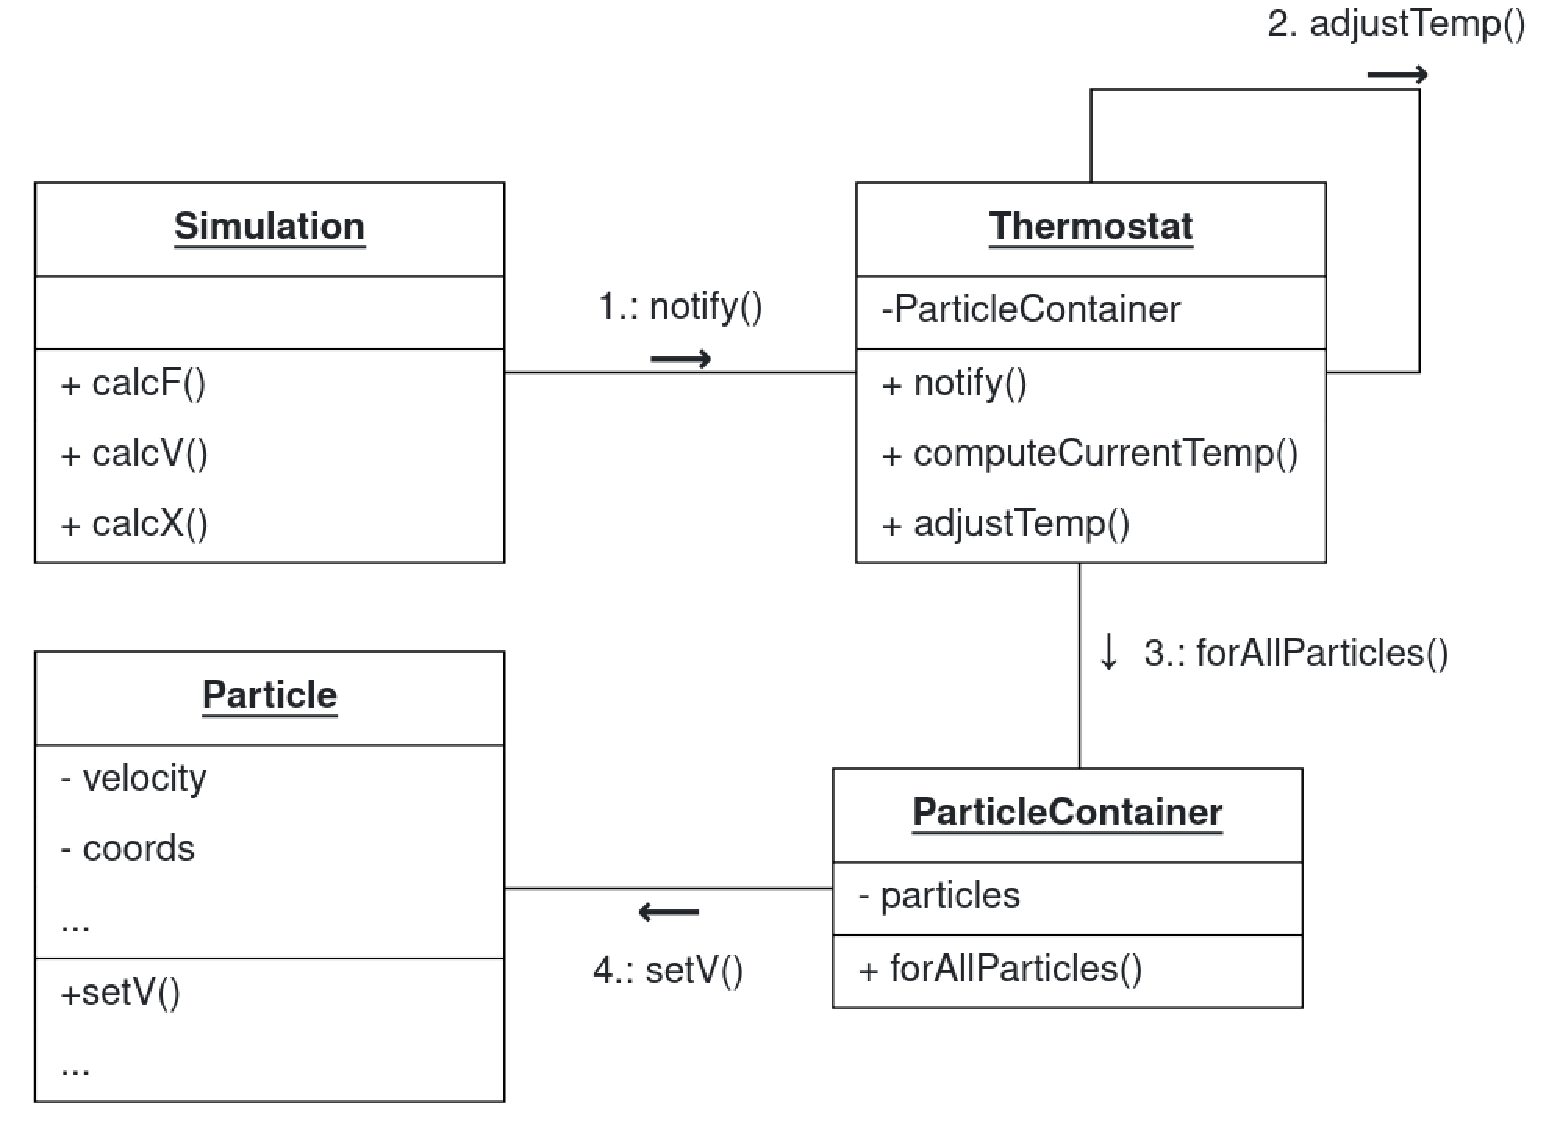
\includegraphics[width=0.55\linewidth]{ThermoComm}
		%\caption{}
		\label{fig:thermocomm}
	\end{figure}
	
	
\end{frame}

\begin{frame}
	\frametitle{Adapting ParticleContainer for periodic bounds}
	\large
	Idea:\\
	\begin{itemize}
		\item Provide virtual cells around the actual domain for anyone who needs it
		\item Existence of additional cells is invisible with old interface
	\end{itemize}
	
	\begin{columns}
		\begin{column}{0.6\textwidth}
			\vspace{-5cm}	
			\begin{figure}
				\centering
				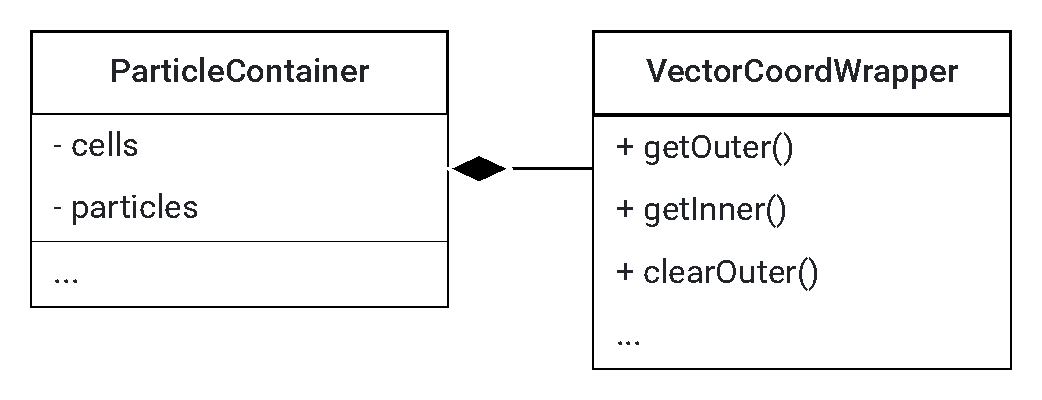
\includegraphics[width=\linewidth]{VectorCoordWrapper}
				\label{fig:vectorcoordwrapper}
			\end{figure}
		\end{column}
		
		\begin{column}{0.3\textwidth}
			\begin{tikzpicture}
				\foreach \x in {1,...,3}{
					\foreach \y in {1,...,3}{
						\draw [draw=black] (\x, \y) rectangle (\x +1 ,\y + 1);
					}
				}
				\foreach \x in {0,...,4}{
					\filldraw [fill=gray, draw=black] (\x, 0) rectangle (\x +1 ,0 + 1);
					\filldraw [fill=gray, draw=black] (\x, 4) rectangle (\x+1, 4+1);
				}
			
				\foreach \y in {1,...,3}{
					\filldraw [fill=gray, draw=black] (0, \y) rectangle (0+1 , \y + 1);
					\filldraw [fill=gray, draw=black] (4, \y) rectangle (4+1, \y+1);
				}
			
				\draw [below] (4.5,1.5) -- (6.5, 0.8) node[below] {Halo};
			\end{tikzpicture}
		\end{column}
	\end{columns}


	
	
	
\end{frame}

\begin{frame}
\frametitle{Boundary conditions}
\large
Idea:
\vspace{-0.5cm}
\begin{enumerate}
	\item Temporarily move all particles next to Boundary of the other side
	\item Let Neighbouring cells interact
\end{enumerate} 

%\resizebox{0.5\textwidth }{0.5\textheight }{
	\begin{tikzpicture}[scale=1.3]
	%define constants
	\def\xLargeArrow{4.5}
	\def\yLargeArrow{1.5}
	\def\LargeArrowLength{2.5}
	\def\offSGrid{7.5}
	\def\arrowStart{0.6}
	\def\arrowEnd{1.9}
	
	\def\scale{1.4}
		
	%draw left grid
	\foreach \y in {0,...,2} {
		\filldraw [fill=green, draw=black] (0, \y) rectangle (0 + 1 ,\y + 1);
	}
	\foreach \x in {1,...,3}{
		\foreach \y in {0,...,2}{
			\draw [draw=black] (\x, \y) rectangle (\x +1 ,\y + 1);
		}
	}
	
	\fill (0.2,1.4) circle[radius=2pt];
	\fill (2.8,1.4) circle[radius=2pt];

	%arrow in between
	\draw[->, line width = 1mm] (\xLargeArrow, \yLargeArrow) -- (\xLargeArrow + \LargeArrowLength, \yLargeArrow);
	

	%draw right grid with left row put to the right
	\foreach \y in {0,...,2} {
		\filldraw [fill=green, draw=black] (\offSGrid + 3, \y) rectangle (\offSGrid + 3 + 1 ,\y + 1);
	}
	\foreach \x in {0,...,2}{
		\foreach \y in {0,...,2}{
			\draw [draw=black] (\offSGrid + \x, \y) rectangle (\offSGrid + \x +1 ,\y + 1);
		}
	}

	
	\fill (\offSGrid + 3 + 0.2,1.4) circle[radius=2pt];
	\fill (\offSGrid - 1 + 2.8,1.4) circle[radius=2pt];
	
	%arrows
	\draw[-triangle 60] (\offSGrid + 3.5, 1.5) -- (\offSGrid + 2.5, 1.5);
	\draw[-triangle 60] (\offSGrid + 3.5, 1.5) -- (\offSGrid + 2.5, 2.5);
	\draw[-triangle 60] (\offSGrid + 3.5, 1.5) -- (\offSGrid + 2.5, 0.5);
	
	
	\end{tikzpicture}
%}

\end{frame}

\begin{frame}
	\frametitle{The result}
	%TODO: insert video
	\begin{figure}[h!]
		\centering    
		\movie[label=show3,width=0.7\textwidth,poster
		,autostart,showcontrols,loop] 
		{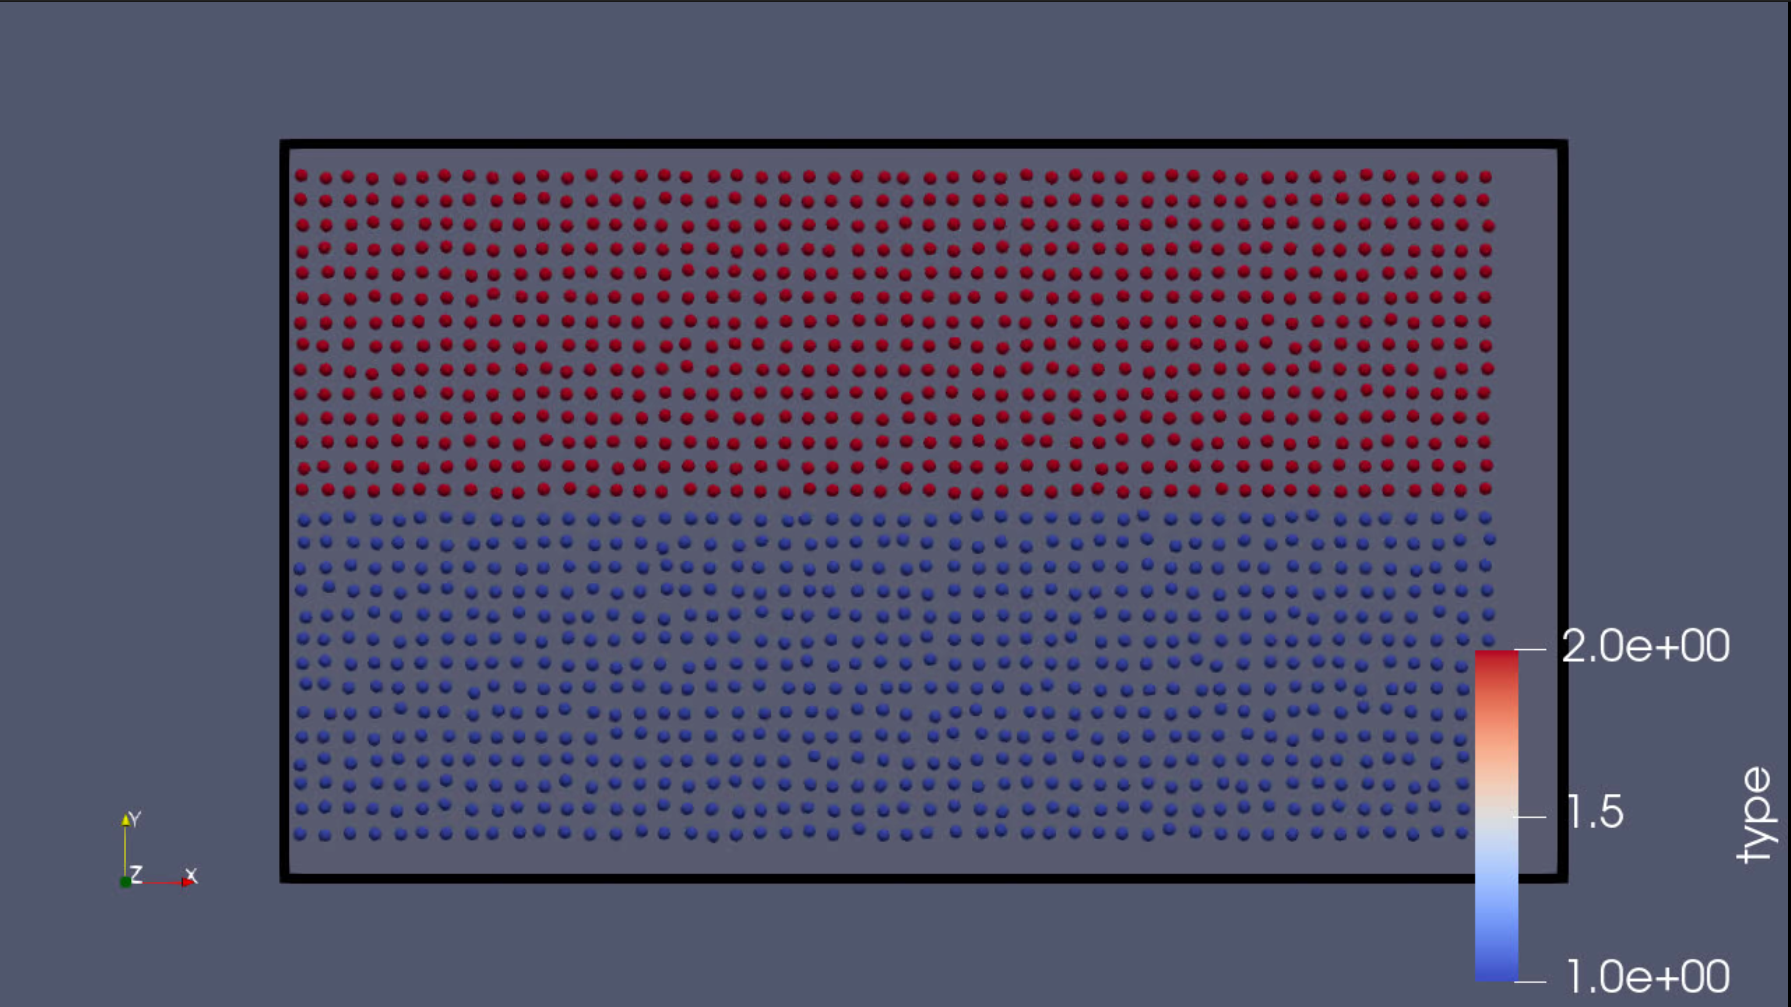
\includegraphics[width=0.7\textwidth]{small_rti.png}}{small_rti_broken.ogx}
		%\caption{caption}
	\end{figure} 
\end{frame}

\begin{frame}
	\frametitle{The problem}
	\large
	\begin{enumerate}
		\item Outer boxes may not have the expected sidelengths
		\item Interacting with neighbouring cells $\centernot \implies$ Catching everything in $r_{cutoff}$
	\end{enumerate}
	
			\begin{tikzpicture}[scale=1.3]
			%define constants
			\def\xLargeArrow{4.5}
			\def\yLargeArrow{1.5}
			\def\LargeArrowLength{2.5}
			\def\offSGrid{7.5}
			\def\arrowStart{0.6}
			\def\arrowEnd{1.9}
			
			\def\scale{1.4}
			
			%draw left grid
			\foreach \y in {0,...,2} {
				\filldraw [fill=green, draw=black] (0, \y) rectangle (0 + 1 ,\y + 1);
			}
			\foreach \x in {1,...,2}{
				\foreach \y in {0,...,2}{
					\draw [draw=black] (\x, \y) rectangle (\x +1 ,\y + 1);
				}
			}
			\foreach \y in {0,..., 2}{
				\draw [draw=black] (3, \y) rectangle (3 + 0.5,\y + 1);
			}
			
			\fill (0.2,1.4) circle[radius=2pt];
			\fill (2.8,1.4) circle[radius=2pt];
			
			%arrow in between
			\draw[->, line width = 1mm] (\xLargeArrow, \yLargeArrow) -- (\xLargeArrow + \LargeArrowLength, \yLargeArrow);
			
			
			%draw right grid with left row put to the right
			\foreach \y in {0,...,2} {
				\filldraw [fill=green, draw=black] (\offSGrid + 3 - 0.5, \y) rectangle (\offSGrid + 3 + 1 - 0.5,\y + 1);
			}
			\foreach \x in {0,...,1}{
				\foreach \y in {0,...,2}{
					\draw [draw=black] (\offSGrid + \x, \y) rectangle (\offSGrid + \x +1 ,\y + 1);
				}
			}
		
			\foreach \y in {0,..., 2}{
				\draw [draw=black] (\offSGrid + 2, \y) rectangle (\offSGrid + 2 + 0.5,\y + 1);
			}
			
			
			\fill (\offSGrid + 3 - 0.5 + 0.2,1.4) circle[radius=2pt];
			\fill (\offSGrid - 1 + 2.8,1.4) circle[radius=2pt];
			
			%arrows
			\draw[-triangle 60] (\offSGrid + 3.5 - 0.5, 1.5) -- (\offSGrid + 2.5 - 0.25, 1.5);
			\draw[-triangle 60] (\offSGrid + 3.5 - 0.5, 1.5) -- (\offSGrid + 2.5 - 0.25, 2.5);
			\draw[-triangle 60] (\offSGrid + 3.5 - 0.5, 1.5) -- (\offSGrid + 2.5 - 0.25, 0.5);
			
			
		\end{tikzpicture}
	
	$\implies$ Interact with one more "`Cellblock"' in that direction
\end{frame}

\begin{frame}
	\frametitle{CI/CD improvements}
	\begin{columns}
		\begin{column}{0.3\textwidth}
			\begin{figure}
				\centering
				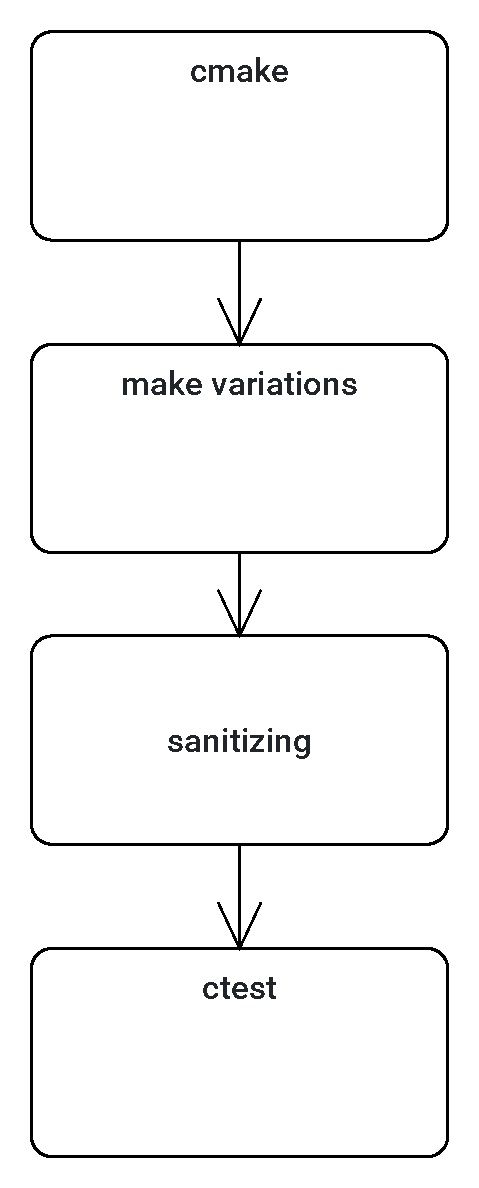
\includegraphics[width=0.55\linewidth]{cicd_old}
				\label{fig:cicdold}
			\end{figure}
			
		\end{column}
	
		\begin{column}{0.7\textwidth}
			\vspace{-1.5cm}
			\begin{figure}
				\centering
				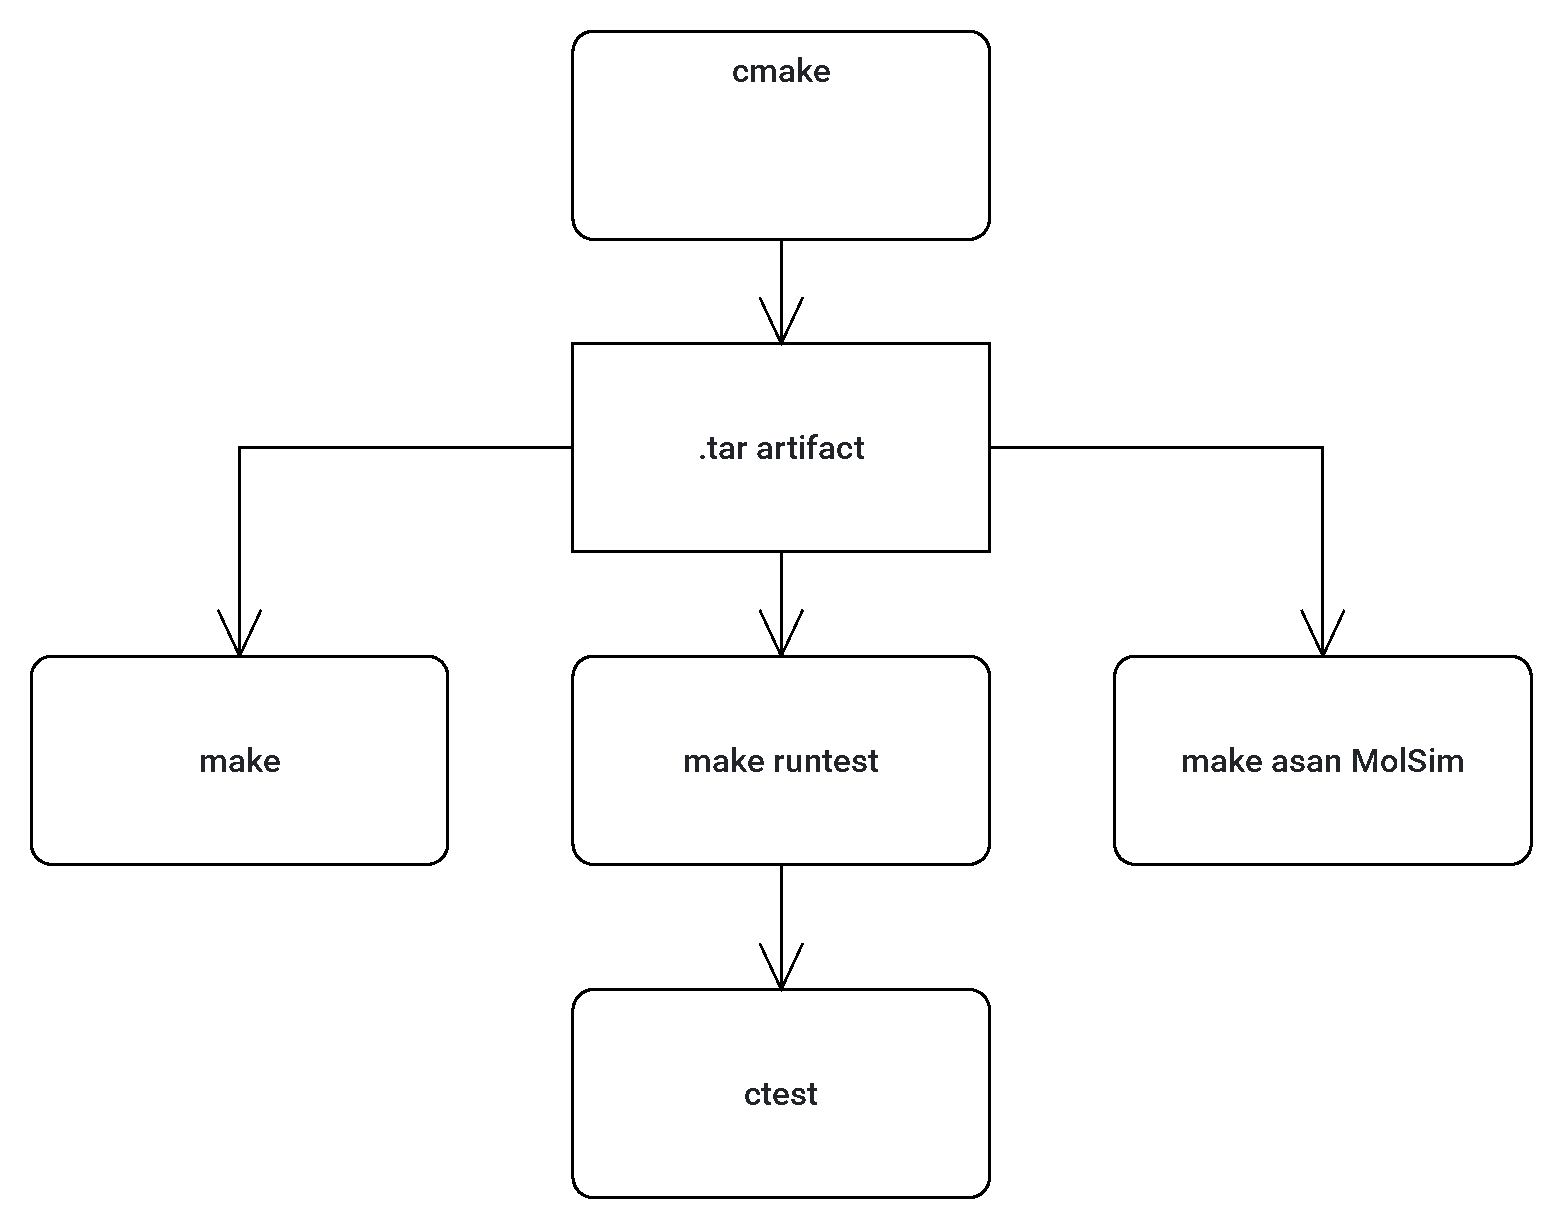
\includegraphics[width=0.8\linewidth]{cicd_new}
				\label{fig:cicdnew}
			\end{figure}
			
		\end{column}
		
	\end{columns}
\end{frame}

\begin{frame}
	\frametitle{Adding Periodic bounds}
	\large
	This slide should look very familiar to Assignment 3
		\begin{figure}
			\centering
			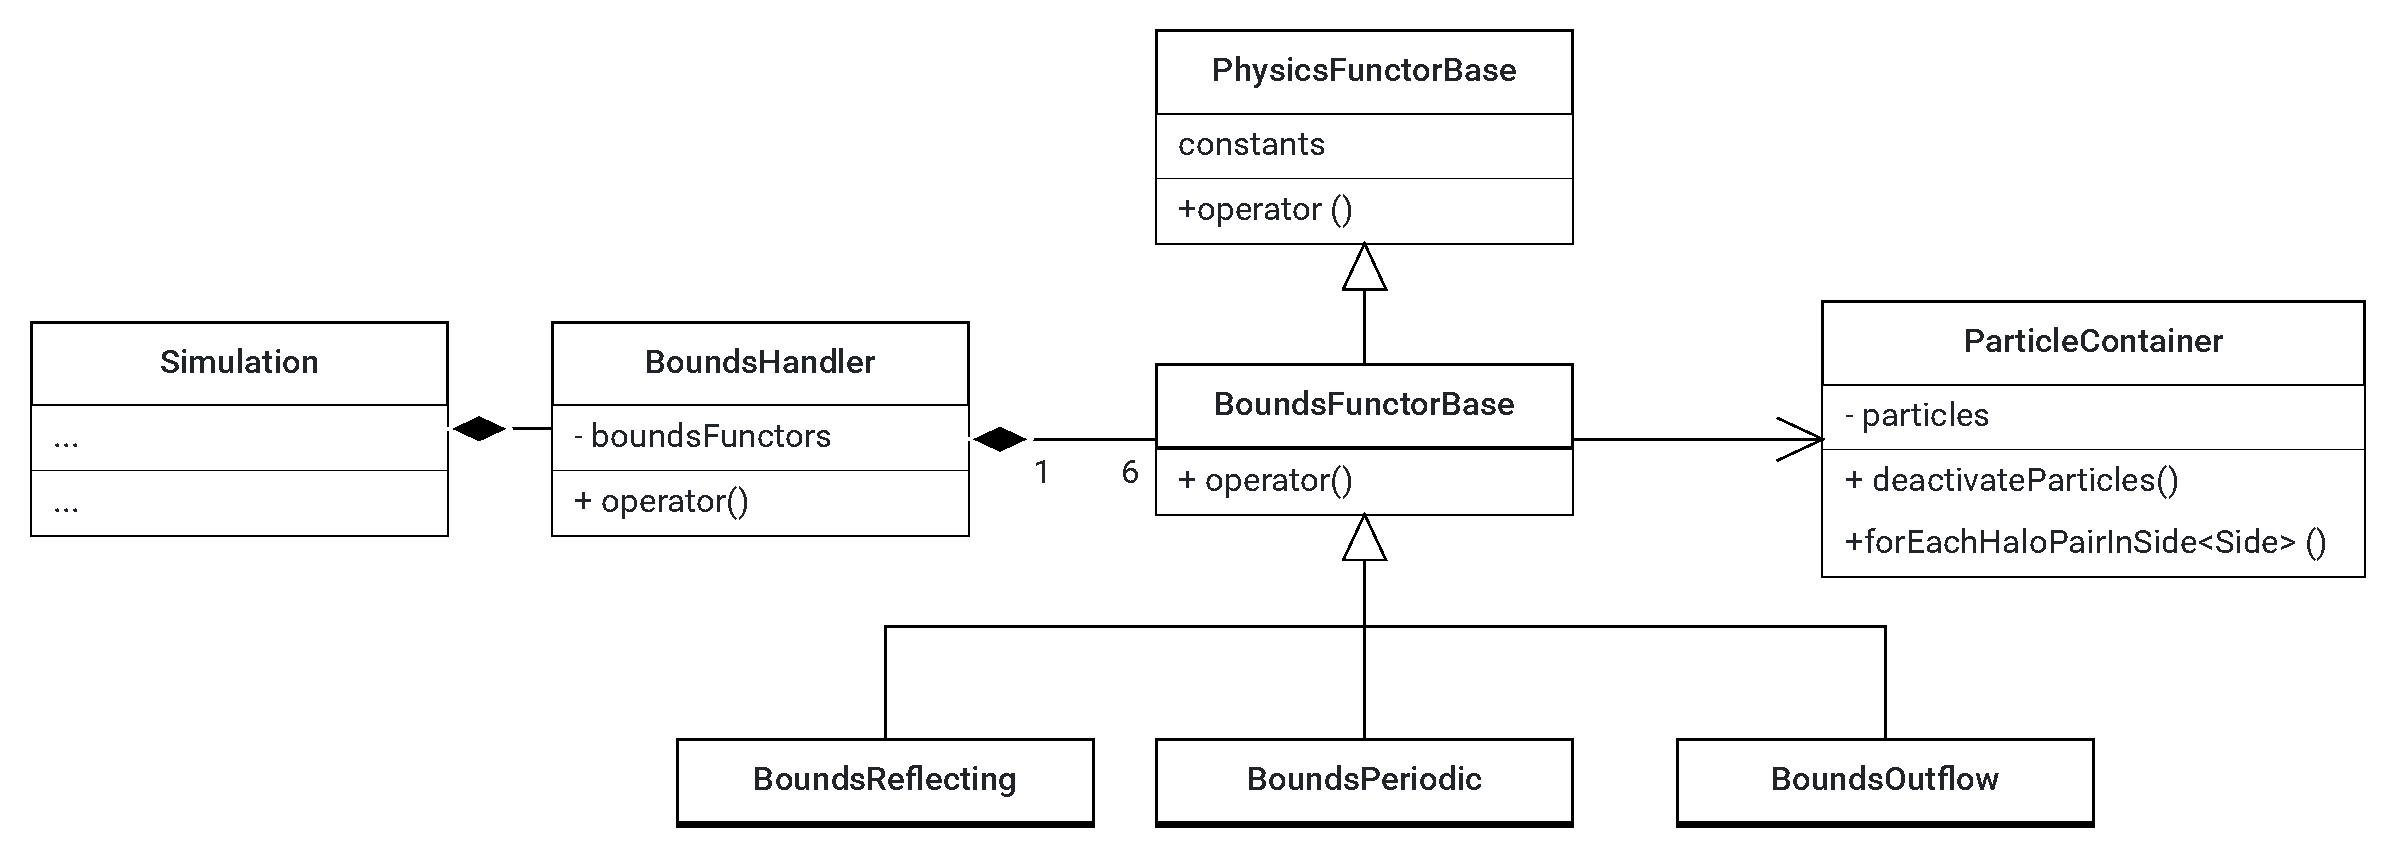
\includegraphics[width=0.95\linewidth]{BoundaryMolSim}
			\label{fig:boundarymolsim}
		\end{figure}
\end{frame}

\begin{frame}[fragile]
	\frametitle{Adding Gravitational Force}
	%\begin{columns}
	%	\begin{column}{0.5\textwidth}
			\begin{figure}
				\centering
				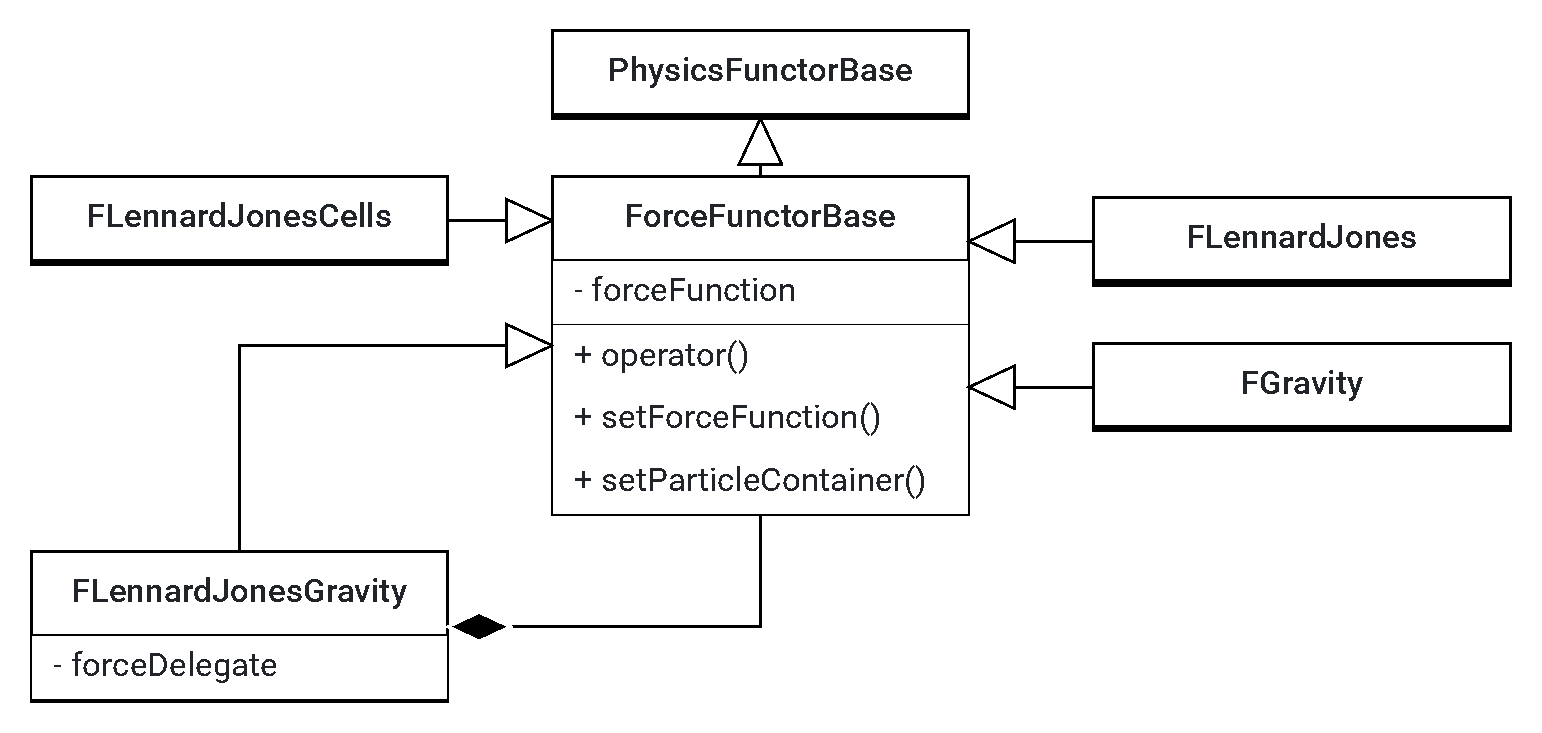
\includegraphics[width=0.6\linewidth]{FGravity_added}
				\label{fig:fgravityadded}
			\end{figure}
	%	\end{column}
	%\begin{column}{0.5\textwidth}
			
\begin{lstlisting}
		FLennardJonesGravity::operator()(){
			forceDelegate->operator()();
			particleContainer.forAllParticles([](auto& p){
			p.force[1] += p.m * gGrav;
			});	}
\end{lstlisting}

	%\end{column}
		
	%\end{columns}
	
	
	
\end{frame}

\begin{frame}
	\frametitle{Rayleigh-Taylor instability}
	\begin{figure}[h!]
		\centering    
		\movie[label=show3,width=0.75\textwidth,poster
		,autostart,showcontrols,loop] 
		{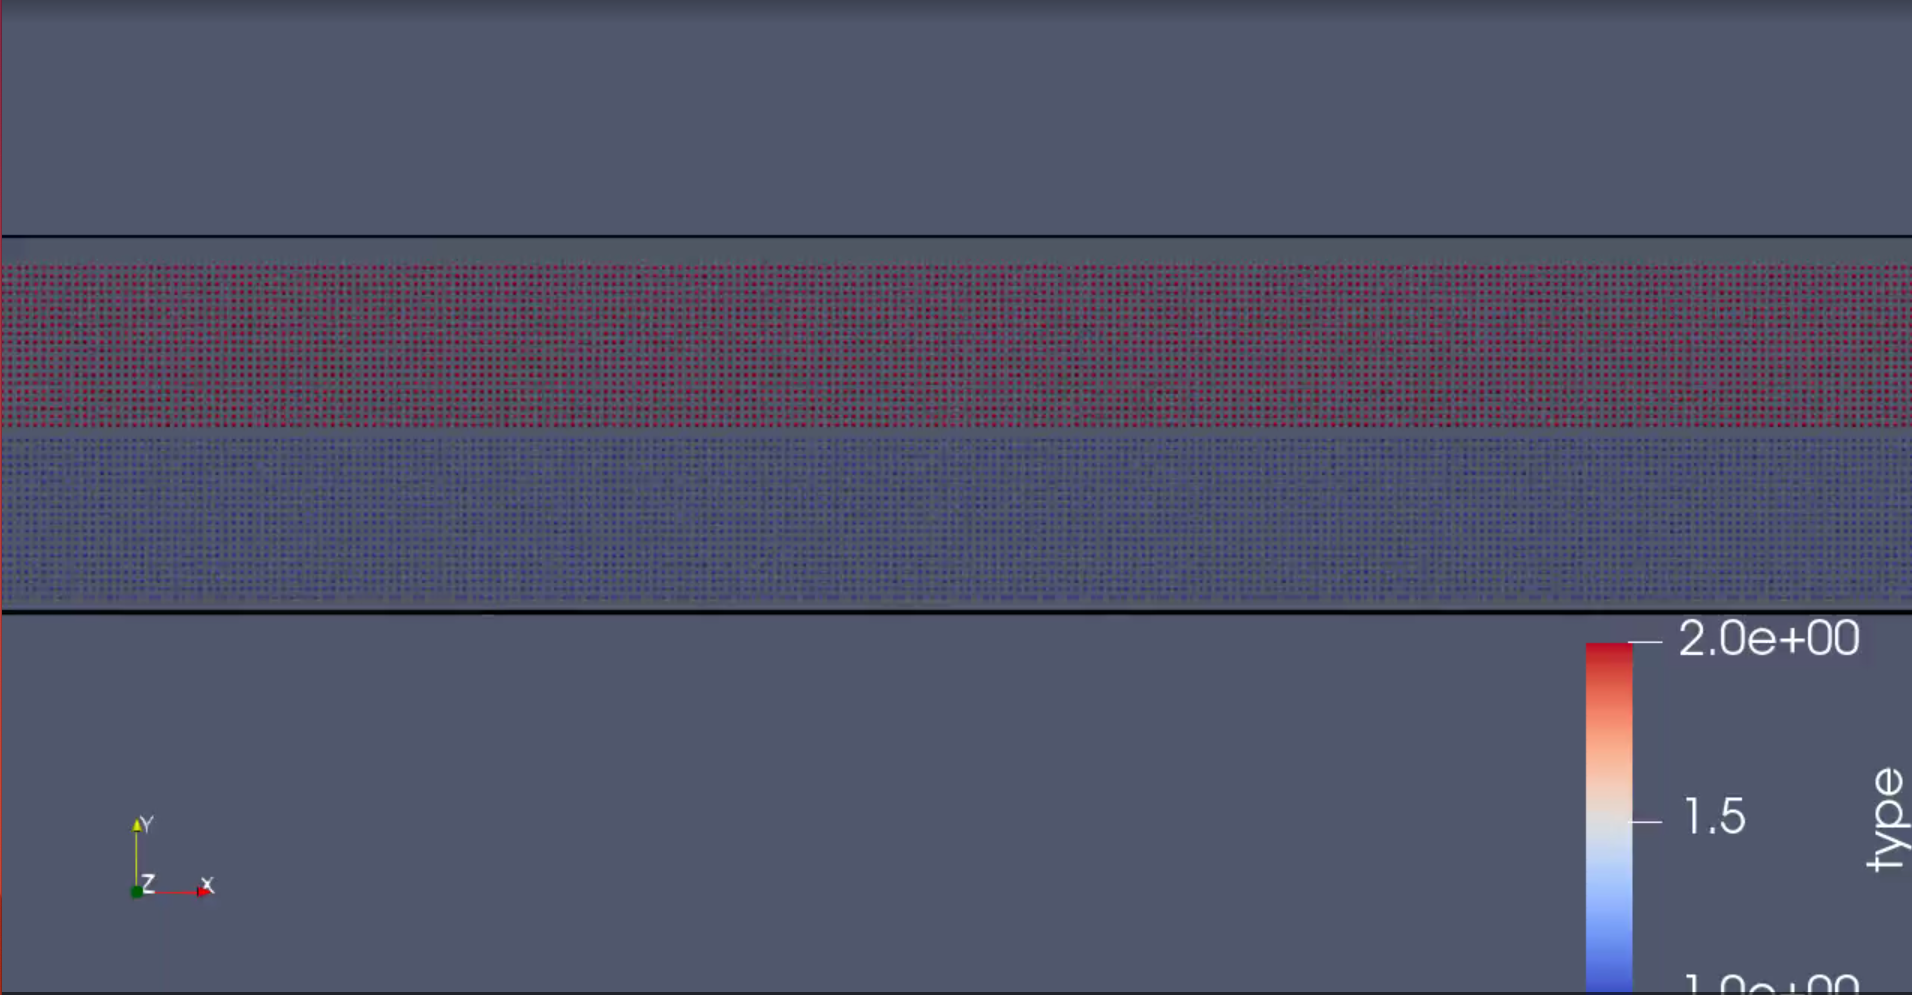
\includegraphics[width=0.75\textwidth]{large_rti.png}}{large_rti.mp4}
		%\caption{caption}
	\end{figure} 
\end{frame}

\begin{frame}
	\frametitle{Falling drop}
	\begin{figure}[h!]
		\centering    
		\movie[label=show3,width=0.70\textwidth,poster
		,autostart,showcontrols,loop] 
		{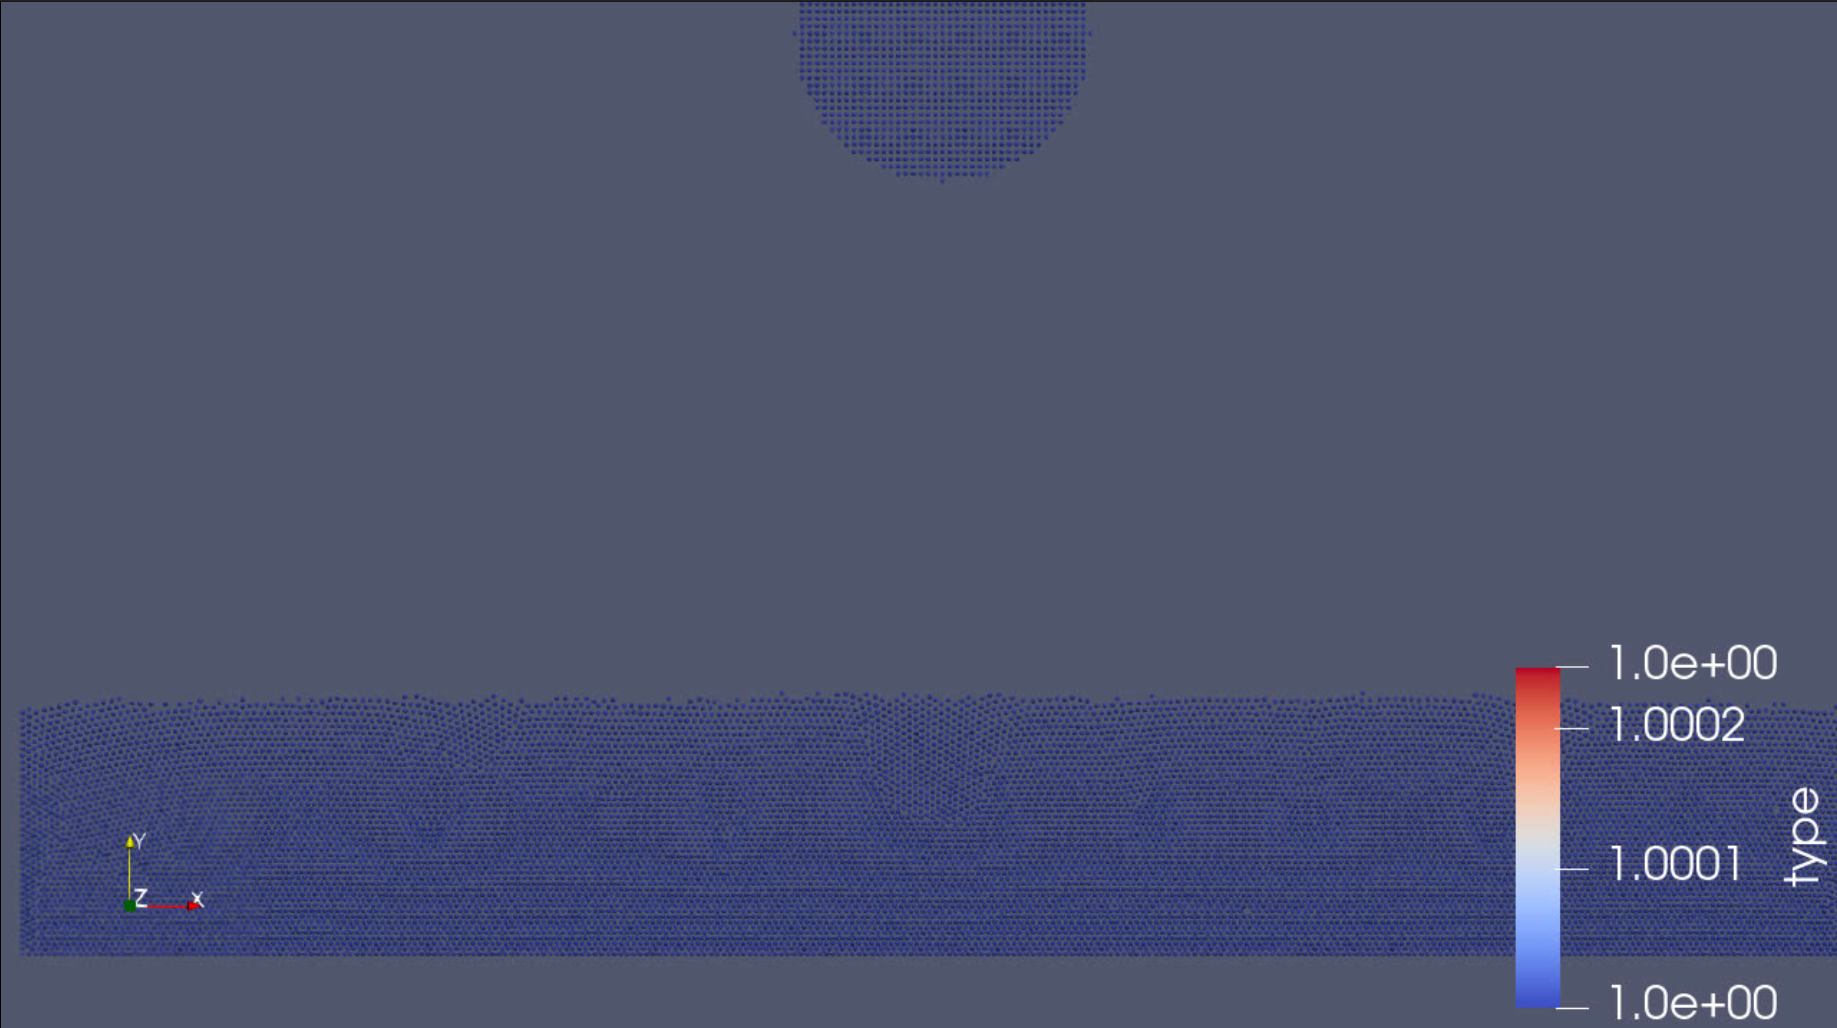
\includegraphics[width=0.70\textwidth]{falling_drop.png}}{falling_drop_out.mp4}
		%\caption{caption}
	\end{figure} 
\end{frame}

\begin{frame}
	\PraesentationBildUhrenturm
	%\PraesentationStartseiteFlaggen
\end{frame}


%\frame[label=blah]{
%	\begin{center}%
%		\href{run:/usr/local/bin/mplayer -fs standard-benchmark.mp4}{
%		\includegraphics[scale=0.25]
%		{Assignment2_Presentation.pdf}}

%		\includemovie{.85\textheight}{.85\textheight}{standard-benchmark.mp4}%
%	\end{center}%
%	\note{%
%		\begin{itemize}
%			\item blah
%			\item blah
%		\end{itemize}
%	}%
%}


%%%%%%%%%%%%%%%%%%%%%%%%%%%%%%%%%%%%%%%%%%%%%%%%%%%%%
%% Folie: Gültigkeit der Masterfolien              %%
%%%%%%%%%%%%%%%%%%%%%%%%%%%%%%%%%%%%%%%%%%%%%%%%%%%%%

%%%%%%%%%%%%%%%%%%%%%%%%%%%%%%%%%%%%%%%%%%%%%%%%%%%%%


%%%%%%%%%%%%%%%%%%%%%%%%%%%%%%%%%%%%%%%%%%%%%%%%%%%%%%%%%%%%%%%%%%%%%%%%%%%%%%%%
% FOLIENSTIL: Standard mit Lehrstuhl-, Fakultäts- und Universitätsnamen im
% Kopfbereich links
\PraesentationMasterKopfzeileDreizeiler

\PraesentationTitelseite


%%%%%%%%%%%%%%%%%%%%%%%%%%%%%%%%%%%%%%%%%%%%%%%%%%%%%%%%%%%%%%%%%%%%%%%%%%%%%%%%
% FOLIENSTIL: Weisse Schrift auf blauem Grund
\PraesentationMasterWeissBlau

%%%%%%%%%%%%%%%%%%%%%%%%%%%%%%%%%%%%%%%%%%%%%%%%%%%%%
%% Startseiten                                     %%

% Setzt die Startseite auf eine mit Flaggen als Hintergrund:
\PraesentationStartseiteFlaggen

% Setzt die Startseite auf eine mit mit einer Zeichnung des TUM-Uhrenturms:
%\PraesentationStartseiteUhrenturm

% Setzt die Startseite auf eine ohne Hintergrund:
%\PraesentationStartseiteLeer

\PraesentationTitelseite % Fügt die Startseite ein
%%%%%%%%%%%%%%%%%%%%%%%%%%%%%%%%%%%%%%%%%%%%%%%%%%%%%


\begin{frame}
    \PraesentationUeberschriftZweizeilig{Präsentationsmuster}{kann auch als Kapiteltrenner verwendet werden}
\end{frame}

%%%%%%%%%%%%%%%%%%%%%%%%%%%%%%%%%%%%%%%%%%%%%%%%%%%%%%%%%%%%%%%%%%%%%%%%%%%%%%%%
% FOLIENSTIL: Weisse Schrift auf schwarzem Grund
\PraesentationMasterWeissSchwarz

\begin{frame}
    \frametitle{Präsentationsmuster}
\end{frame}


%%%%%%%%%%%%%%%%%%%%%%%%%%%%%%%%%%%%%%%%%%%%%%%%%%%%%%%%%%%%%%%%%%%%%%%%%%%%%%%%
\end{document} % !!! NICHT ENTFERNEN !!!
%%%%%%%%%%%%%%%%%%%%%%%%%%%%%%%%%%%%%%%%%%%%%%%%%%%%%%%%%%%%%%%%%%%%%%%%%%%%%%%%

